\documentclass{llncs}
\usepackage{graphicx}
\usepackage{float}
\usepackage{fancyvrb}
\usepackage{fancyhdr}

% page numbering
\pagestyle{fancy}
\fancyhf{}
\fancyhead[LE]{\thepage} % Left side on Even pages
\fancyhead[RO]{\thepage} % Right side on Odd pages
\renewcommand{\headrulewidth}{0pt} % remove header line

\title{CI/CD for Python}
\author{Robin Sonner}
\institute{University Freiburg, Freiburg, Germany}

\begin{document}

\maketitle

\section{Introduction}

Continuous Integration (CI) and Continuous Deployment (CD) are established practices in modern software engineering aimed at improving software quality, reliability, and delivery speed. Continuous Integration is the automated process of regularly integrating code changes into a shared repository, where each integration is verified through automated builds and tests. Continuous Deployment is the process of automatically delivering validated changes to production or release environments. These practices have emerged from agile software development and DevOps methodologies to reduce integration problems, improve feedback cycles, and increase development productivity \cite{shahin2017}.

The theoretical foundations of CI/CD were established by Fowler and Foemmel \cite{fowler2006}, who defined ten core practices intended to increase the speed of software development feedback cycles and improve software quality. These practices span source code management, build automation, testing, environment configuration, system visibility, and deployment.

In the project, a Weather Application and a Python library were developed together with two CI/CD pipelines implemented using Jenkins and GitHub Actions. The report mainly addresses the following questions:

\begin{itemize}
\item What can a CI/CD pipeline provide for Python projects (Section 2)?
\item How do Jenkins and GitHub Actions compare as CI/CD platforms (Section 3)?
\end{itemize}

Considering that the Application displays weather information in the form of charts, it's also beneficial to explore chart creation in python. The graphical user interface uses PyQt6, which pairs well with PyQtGraph. Section 4 outlines the creation of a usage demonstration for PyQtGraph to generate the Dual-Axis Temperature/Precipitation charts displayed in the application. 


\section{CI/CD for Python}

The Jenkins Pipeline and GitHub Actions Pipeline were written to perform exactly the same tasks. Both Pipelines address the development of a python application and a library package. The Pipelines can be divided into Continuous Integration and Continuous delivery segments.

\paragraph{Continuous Integration.} High Quality code makes future work  easier, so we want to only integrate high quality code to the repository. What is high quality code is a complex topic. However there are a few automated checks that can provide partial coverage of the aspects of high quality. These checks do not guarantee quality, but failing them reveals improvement opportunities. 
I use the linter flake8 to identify syntax errors, logic mistakes and deviations from PEP 8 (Style Guide for Python). The error E501 (long lines) is disabled \footnote{Personal Preference: In the cases where black does not reformat long lines, I want my linter to accept them as well}. The formatters black and isort ensure consistent code formatting and import ordering.

Functional correctness is checked using the unittest framework. Test cases are automatically discovered and executed during each pipeline run, allowing bugs to be caught early.

To allow other people to use the projects library, it must be documented. For Python (and a few other languages) sphinx can auto-generate documentation based on docstrings and specially formatted comments. Letting Sphinx run as part of the CI-Pipeline ensures that incompatible docstrings are caught early, as opposed to only during release creation. The code must run on Linux and Windows with Python 3.13 and 3.14, requiring the pipeline to test all four combinations.

\paragraph{Continuous Deployment.} The project deploys both an application and a library package. I use annotated tags to trigger releases, with tag names specifying version numbers and annotations providing release messages.
Python code executes without compilation but requires a compatible interpreter and dependencies. Application deployment packages the interpreter and dependencies with the source code to create executables. The pyinstaller tool performs this packaging. Outside of development I normally use windows. Therefore, the weather application releases as a Windows executable. Linux releases would follow the same procedure. Built executables are published as GitHub releases.

Python packages typically distribute via PyPI, enabling installation through pip. This project uses TestPyPI (\footnote{\url{https://test.pypi.org/}}), which mirrors PyPI functionality without affecting the production Package Index. The package's limited scope (primarily CI/CD exploration) offers minimal utility to external users. Should the project be further expanded release to PyPI could be considered.

Package documentation hosts on ReadTheDocs\footnote{\url{https://readthedocs.io/}}. Documentation deployment to ReadTheDocs occurs outside CI/CD automation, as the platform builds documentation independently. The platform uses sphinx to build the documentation. Pipeline-verified Sphinx compatibility ensures ReadTheDocs can build correctly. ReadTheDocs is free only for public repositories. A public repository\footnote{\url{https://github.com/Robin-Sonner/do-I-need-an-umbrella}} mirroring the code from the private GitHub classroom repository was created for usage of ReadTheDocs.


\section{Jenkins and GitHub Actions}

Jenkins and GitHub Actions represent two widely adopted CI/CD platforms capable of providing the functionalities described in Section 2. Jenkins \footnote{\url{https://www.jenkins.io/}}, an open-source automation server released in 2011, supports self-hosted and managed deployments. GitHub Actions\footnote{\url{https://github.com/features/actions}}, introduced in 2019 is a proprietary solution deeply integrated with GitHub repositories.

\paragraph{Setup.} GitHub provides hosted runners for Windows and Linux with preconfigured Python versions. A test matrix spanning multiple operating systems (Linux, Windows) and Python versions (3.13, 3.14) can therefore simply be specified in pipeline configurations, with GitHub managing all of the needed infrastructure. Hosted runners are provided at no cost for public repositories and a free tier of 2000 minutes of runner usage per month is offered for private repositories.

The Jenkins instance was self-hosted. Due to the complexity of the final requirements (multiple operating systems and python versions) an iterative approach was chosen. Initially the Jenkins Server was directly installed on a Windows 10 host machine, using the built-in node as pipeline executor. This configuration presents security risks: malicious shell commands injected into pipeline code execute with host privileges, exploitable by any contributor with repository write access. Platform constraints limited testing to the host environment, disallowing testing on Linux verification. 

Jenkins was later reinstalled as a Docker Container. This time two permanent agents (Linux and Windows hosts) were set up and the built-in node disabled. The Jenkins server then only orchestrated pipeline execution across the two agents. Due to the Agents different operating system (Windows10 and Linux Mint) and both having Python 3.13 and 3.14 set up, the required matrix testing was now executed. Future enhancement would replace permanent agents with dynamic agents, created from templates (e.g., Dockerfiles) and destroyed post-execution. Due to time constraints this step wasn't taken.

\paragraph{Trigger Mechanisms.} 
GitHub Actions triggers automatically on repository push events without additional configuration. If needed trigger conditions can be customized. 
Jenkins supports multiple trigger mechanisms with GitHub webhooks providing the most elegant solution. These trigger automatically on every push without client-side configuration. Webhook integration requires exposing the Jenkins instance to external networks. To avoid threatening the security of the (private) network and computer, this wasn’t done. Instead, Jenkins was configured to accept external triggers using a provided token. On my development machines Git hooks were set up as this external trigger, executing the following script:

\begin{Verbatim}
#!/bin/bash
curl -X POST http://HOST_IP_ADDRESS:8080/job/dinau-pipeline/build \
    --user robin:JENKINS_TOKEN
\end{Verbatim}

The Initial implementation used post-commit hooks, later replaced with pre-push hooks. Pre-push hooks trigger on both commit and tag pushes, allowing for tags to be used as release trigger. Post-commit hooks execute only during commit creation.

\paragraph{Pipeline Definition.}
GitHub Actions pipelines are defined in YAML files within the .github/workflows directory. The YAML syntax supports embedded shell command blocks. The Syntax is indentation based, which I personally prefer over bracket based syntax. Secrets (e.g., \texttt{TESTPYPI\_TOKEN}) are configured in repository settings and accessed in the pipeline as follows:
\begin{Verbatim}
    env:
        TESTPYPI_TOKEN: ${{ secrets.TESTPYPI_TOKEN }}
    run: |
        some code that uses $TESTPYPI_TOKEN
\end{Verbatim}

Jenkins provides multiple automation approaches: freestyle projects, single-branch pipelines, and multi-branch pipelines (ordered by complexity). This project implements single-branch pipeline configuration. Pipelines are defined either through the web interface or Jenkinsfile, the latter was selected for reproducibility. Pipeline code uses Groovy\footnote{\url{https://groovy-lang.org/}} which is Java-like and uses a bracket syntax making indentations optional. Groovy executes within a sandbox that restricts method access to a deemed safe subset. Embedded shell commands execute outside the sandbox and could contain malicious code. Secrets are configured in the Jenkins Credential store and can be accessed in the pipeline as follows:
\begin{Verbatim}
    withCredentials([
        string(credentialsId: 'TestPyPIToken', variable: 'TESTPYPI_TOKEN')
    ]) {
        some code that uses ${env.TESTPYPI_TOKEN}
    } 
\end{Verbatim}
Groovy syntax is less readable than GitHub Actions YAML Syntax, primarily due to backslash escape requirements (backslash is the escape character of groovy). The pipeline implementation uses manual GitHub API calls for status notifications and artifact uploads. Plug-ins like GitHub Checks \footnote{\url{https://plugins.jenkins.io/github-checks/}} could simplify this, but need the Jenkins instance to be authenticated as a GitHub App, requiring it to be exposed outside of the network.

\paragraph{Plugin Ecosystem.}
Jenkins provides an extensive plugin system enabling integration with numerous source control platforms (GitHub, GitLab, Bitbucket, Gitea, SVN) through dedicated plugins. Other plugins can modify the UI, and enable additional functionalities such as dynamic agent creation via Docker Templates. In the project the Blue Ocean plugin was used to modify the UI, creating a Pipeline visualisation which the default Jenkins UI lacks. GitHub Actions features no comparable plugin architecture. Limited Extensibility is supported through community-created actions which can be invoked within pipelines (e.g., \texttt{uses: actions/setup-python@v5}). GitHub Actions are tightly integrated in GitHub repositories, creating a vendor lock-in.


\section{PyQtGraph}
The application supports both PyQtGraph and Matplotlib as interchangeable chart backends, selectable via application settings. Originally comparing these two was considered. This was not done in favour of creating a usage demonstration instead. PyQtGraph was chosen over Matplotlib due to the greater implementation complexity it needs to produce an equivalent chart. 

For demonstration purposes a Jupyter notebook is well suited. It allows for the code to be extended (and the chart to be improved) progressively with each block of the notebook. The code block results persist in the notebook, not requiring re-execution each time the user wants to see the result. 

PyQtGraph is designed for integration within PyQt applications and does not natively support Jupyter rendering. However, a small PyQt application can be launched from within a notebook. The graph can then be displayed in an external Qt window of this application. This approach has the disadvantage of the output not persisting in the notebook.

The most complex chart in the application is the temperature/precipitation chart displayed in the current weather and weather forecast tabs. This chart combines two temperature line plots with a precipitation bar chart on independent y-axes. In Matplotlib, dual-axis charts can be easily created as follows:
\begin{Verbatim}
fig, ax1 = plt.subplots()
ax2 = ax1.twinx()
ax1.plot(hours, temperature, label='Temperature')
ax1.plot(hours, feels_like, label='Feels like')
ax2.bar(hours, precipitation, alpha=0.3, label='Precipitation')
\end{Verbatim}

PyQtGraph needs an additional ViewBox instance to replicate this layout. A further complication arises from the independent auto-scaling of each axis: grid lines of the two y-axes misalign when axes scale independently. Manual axis scaling resolves the misalignment. Interactivity allows the user to revert to auto scaling, so interactivity was disabled. Interactivity is not needed for the application, so this trade-off is acceptable.

\begin{figure}[H]
\begin{center}
  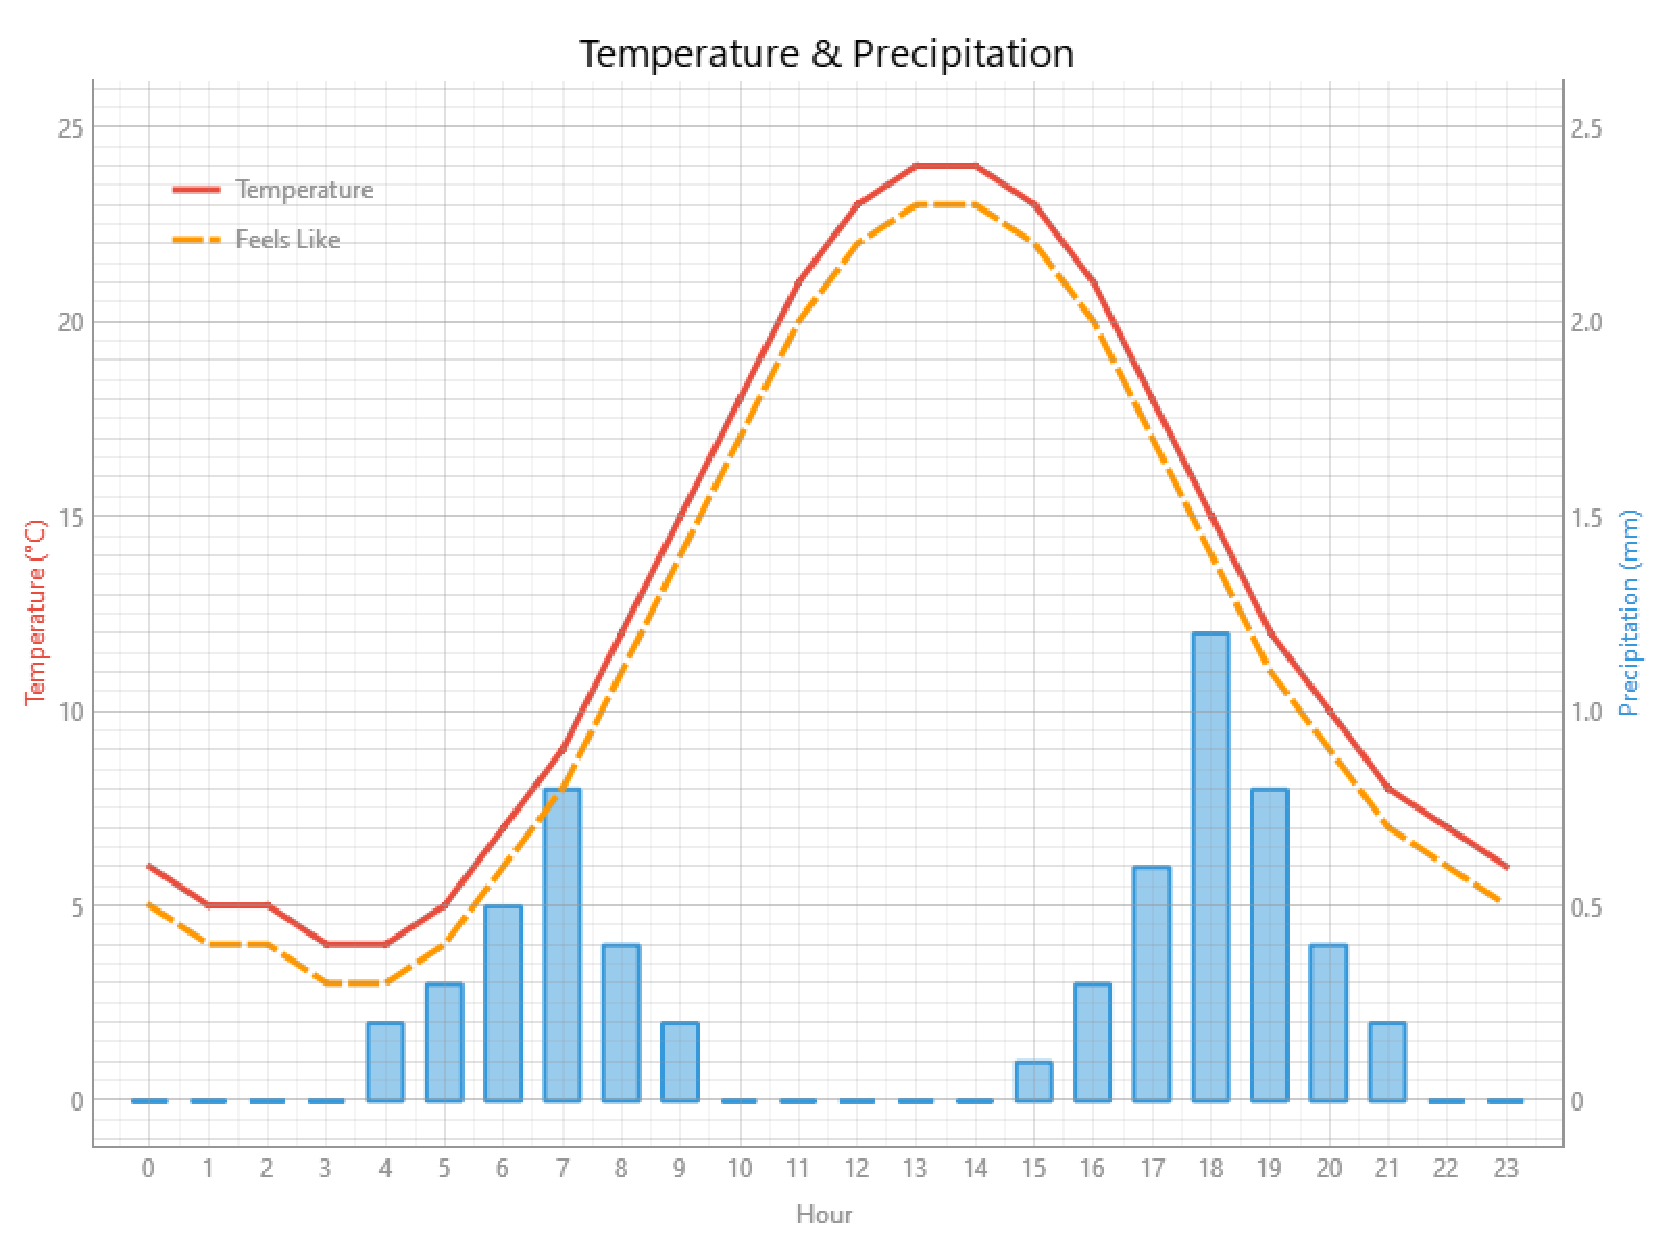
\includegraphics[scale=0.4]{chart.eps}
  \caption{Temperature \& Precipitation Chart rendered with PyQtGraph}
  \label{fig:chart}
\end{center}
\end{figure}

Figure \ref{fig:chart} shows the result of the last code example in the Jupyter notebook.

\section{Most interesting results}
A minimal Jenkins setup installed directly on a host machine using the built-in node needs about 15 minutes from download to first pipeline configuration. This setup carries a few limitations: pipeline code executes with host-level privileges (security risk), testing is restricted to the host operating system, and processing capacity is limited by the server handling all jobs without delegation to potentially remote agents. For getting started into CI/CD none of these restrictions are particularly relevant.

More advanced setups (e.g. Jenkins Server via Docker, multiple agents, potentially even dynamically created agents based on docker templates) require much more time, but are needed to mitigate the mentioned limitations for professional development. GitHub Actions are even simpler to use, needing only the definition of a pipeline, with GitHub taking care of the infrastructure. GitHub Actions does create a Vendor-Lock in and the continued availability of all features for free is not guaranteed. 

Jenkins can be used with a wide range of Source control system. It's usage also extends software development. Freestyle projects support arbitrary PowerShell and Bash script execution with time-based and external event triggers, enabling the automation of a variety of tasks (e.g. automatic creation of backups).

In regards to the application there are two interesting results.
The cell by cell structure of Jupyter notebooks allows to increase the complexity of the example gradually and while they are not designed for executing GUI applications, they can be configured to support that. This allows for demonstrations of libraries tightly coupled to application frameworks, in this case PyQtGraph.
The second finding is that the Open-Meteo API offers an extensive range of weather information, alongside air quality data, marine data, and a historical weather database. Furthermore it's Web UI can generate Python example code for any possible API call. The application uses only a small subset of the Open-Meteo API's capabilities.


\section{Conclusion}

The CI/CD pipeline created in the project shows that the integration and deployment tasks of Python projects can be automated. On the integration side, tools such as flake8, black, and isort ensure consistent code style and catch syntax errors, and the automatic execution of unittests guards against bugs. Sphinx is run as part of the continuous integration to ensure documentation remains buildable at all times. For deployment pyinstaller can packages the application into a self-contained executable, and built packages can be automatically deployed to PyPI or in this case TestPyPI. This leads to increased confidence in every change integrated into the repository and little manual effort for releases.

The project compared Jenkins to GitHub Actions. GitHub Actions advantage lies in its simplicity of use, needing no setup beyond defining the pipeline and configuring its secrets. A self hosted Jenkins instance needs much more work to set up and to maintain. Its advantage lies in its versatility integrating with a broad range of source control systems and being a more general automation platform capable of a wide variety of tasks. 

The project features a PyQtGraph usage demonstration. Jupyter notebooks cell structure was found to be well suited for usage demonstrations, allowing for code examples with progressively increased complexity. This allowed building up to complex result with previous simpler steps ensuring the viewer isn't overwhelmed. Despite PyQtGraph's deep integration into the PyQt Framework its usage can still be demonstrated in a Jupyter notebooks needing only the activation of qt's eventloop and a few lines of support code to create a small QtApplication.


\bibliographystyle{unsrt}
\bibliography{references}

\begin{tabular}{@{}p{3cm}|p{10cm}@{}}

\textbf{Topics}  \\
\hline
Linux & The CI/CD Pipelines are partially executed under Linux, but there is nothing noteworthy to report. \\
Text editor & There is nothing to report.\\
Git & Git was used as version control system. The project focuses on the development of a CI/CD Pipeline for Python (section 2) and the Comparison of CI/CD Platforms that can be used to create said pipeline (section 3) \\
Docker & Jenkins server was containerized using Docker. A Dockerfile is provided to allow others to easily install and view the developed application and the Jupyter notebook containing the PyQtGraph usage example. No further research on docker was done and there is nothing to report. \\
Automation & I find the CI/CD to be more suited in the git category, so I counted it there. Apart from that no other automation was done. \\
Plots & The application uses matplotlib and PyQtGraph to generate its charts. The usage of PyQtGraph was found to be more difficult. A usage example of it was created in a jupyter notebook, rendering the dual-axis temperature/precipitation charts used in the application (Section 4)\\
\LaTeX & This report was written in \LaTeX, but there is nothing to report. \\
LLM & There is nothing to report.
\end{tabular}

\end{document}
